\section{Introduction}



\section{}

% \subsection{How is the traveller using social media to talk about his trip?}
\subsection{Traveller's use of social media to talk about his trip}


A traveller\textquotesingle s use of social media can be divided into three phases: before, during and after the trip. \cite{cox2009role} found the predominant use of social media to research about his trip, read more about the destinations and viewing the user generated content (UGC). However, they are not found to be actively participating by creating content. This phase hence mostly involves searching for ideas for probable destinations, planning the trip itinerary, looking up options for accommodation, and opportunities for excursions and other leisure activities\cite{cox2009role}; \cite{fotis2012social}. The use of social media before travelling helps to generate ideas, and helps to imagine how places will be like, reducing the possibilities of risks involved in the process.

It has been found that a traveller\textquotesingle s use of social media for travel purposes, during the trip is much lower than its use before the trip \cite{cox2009role}; \cite{fotis2012social}. While \cite{fotis2012social} shows that 30\% of the respondents searched for travel-related information during their vacations, in Cox et al.\cite{cox2009role} the percentage was seen to be reduced to 6\%. During this period, travellers not only search for travel-related information but also share information regarding their travel with the help of photos, videos, reviews etc \cite{Text100, 2013}. However, the amount of social media content produced during this phase has been found to be much lower than the consumption of social media resources \cite{fotis2012social}. It can be found that social media geo-location sites such as Foursquare provides discounts and coupons to travellers by encouraging them to use social media during this phase, thus fostering tourism and hospitality businesses \cite{hudson2013impact}.

Travellers use social media after the trip to post information regarding their trip. This can be in the form of comments, reviews, photos or pictures \cite{fotis2012social}\cite{parra2012travellers}. This content is known as the user generated content(UGC) \cite{simms2012online}. Social media producing takes place during this phase. This production encompasses the creation and publication of an individual's personal contents like texts, images, audio and video \cite{Shao, 2009}. The evidence of social media’s importance in the travel context from different sources can be summarised as the following. While social media websites in the United Kingdom are the main resource for planning a holiday \cite{World Travel Market, 2013}, 44\% of leisure travellers in Asia Pacific region use social media platforms to seek advice and as inspiration regarding their choice of travel destinations \cite{eMarketer, 2013}. According to a study performed by TripAdvisor\textquotesingle s TripBarometer \cite{2014b}, online travel reviews influence 89\% of the travellers around the globe while they are choosing their accommodation. Mediabistro, 2012 shows that more than 50\% of the travellers actually change their original travel plans after browsing through social media websites.

A significant number of studies have shown that in addition to the informational benefits of social media, reading travel reviews made the trip planning process fun and enjoyable and got the travellers more excited about travelling \cite{10.1007/978-3-211-77280-5_4}\cite{gretzel2007online} \cite{parra2012travellers}. Users from online travel communities such as TripAdvisor.com or VirtualTourist.com indulged in online community activities for informational as well as hedonic benefits \cite{chung2008web}. \cite{doi:10.1177/0047287503258824} pointed out that the hedonic needs played an important role in predicting the level of participation of a traveller in an online travel community. Positive relationships have been established between the perceived hedonic benefits and the intention to use social media for travel planning by \cite{ayeh2013predicting}.  Perceived enjoyment also can be used as a determinant of creating travel content online. It was found by \cite{YOO2011609} that enjoyment is capable of driving the creation of travel content generated media. A more recent study by \cite{doi:10.1080/10548408.2013.751237} affirmed the above conclusion by stating that perceived enjoyment not only had a positive relationship with the use of social media for travel planning but also affected the actual creation of travel content online.
All these studies show empirical evidence of how individuals use travel-related social media for both information and hedonic purposes. The personalization of information search, with the advent of Web 2.0 also contributes to its hedonic value \cite{doi:10.1080/14616688.2012.762542}.

Several studies \cite{chiu2012china}\cite{foster2011exploring}\cite{kurtulucs2015social} performed a cluster analysis to identify the different segments of travellers. It identified three broad groups - the social enthusiasts, the participators and the inactives. Specifically, the study by \cite{amaro2016travelers} finds five segments that are capable of distinguishing social media users according to their degree of involvement in consumption and generation of travel contents. No particular difference has been found among these segments based on gender or national travel experience, however, the number of international trips has been found to be significantly lower in the inactive cluster. This study also reports a higher percentage of travellers who purchase travel online in the segments characterized by more involvement with travel content on social media. Significant differences were also spotted with respect to other aspects, namely, age, perceived enjoyment and social media involvement. 	The percentage of travellers using online websites to purchase travel services is smaller in the inactive segment (51\%), followed by segment 2 and 3 (60\% and 62\%, respectively), and finally segments 4 and 5 with 70\% and 69\%, respectively.
These results from \cite{amaro2016travelers} provide useful insights to travel online marketers and social media websites providers who need to be aware of the different segments in order to customize their websites accordingly.

It can be concluded from \cite{amaro2016travelers} that fully engaged social media users, as well as occasional consumer and creators, the two segments with a higher level of social media creation, are comprised of younger travellers who perceive higher levels of enjoyment with the use of social media for travel purposes and are also more involved with social media websites. The importance of these segments to online travel providers can be accorded to their participation in creating travel related content, to influence others and, in turn, affect travel decisions.

\cite{pan2012theoretical}\cite{YOO2011609} show that the people consuming travel information are significantly higher than people generating it.  

While \cite{ip2012profiling} found that creation of online travel content increased with education level until university level and then decreased, \cite{yoo2016use} study found no significant differences, between travel social media creators and non- creators, in terms of education. The findings of \cite{maro2016travelers} clarify this issue. The correlation between the higher education level, doctoral degree, and lesser creation of travel content can be attributed to ageing and time restrictions, as higher educational levels are associated with older age classes and higher level jobs which in turn is associated with lower levels of social media creation. 

		


% \subsection{What are the factors behind a travellers’ engagement in travel-related social media?}
\subsection{Factors governing a traveller\textquotesingle s engagement in travel-related social media}

 The bridge between the number of users and the number of actual content creators remains large even though there has been an increase in the number of travellers engaging themselves in consumer-generated media (CGM) use and creation, making it important to find out the driving force behind this minority of creators and what makes them different from those who only use CGM. \cite{yoo2011influence}

Even though numerous personal characteristics have been examined in consumer behaviour research, a traveller\textquotesingle s personality has been found to be a particularly influential trait that is capable of predicting behaviour over time and across various situations \cite{woszczynski2002exploring}.  \cite{yoo2011influence} further investigated the impact of personality on travel CGM creation and the results indicate that travellers\textquotesingle personality traits have a significant influence on perceived barriers to content creation, motivations to engage in CGM creation, and other specific creation behaviours. \cite{acar2007online}; \cite{tuten2001understanding} suggest that the personality of an individual also plays an important role in predicting different online behaviours.

 
\cite{wang2002defining} demonstrated that levels of participation in online tourist communities can be explained in terms of the fulfilment of needs. They proposed that tourists who participate in online tourist communities are motivated by functional, social and psychological needs. While travellers collect and consume information to satiate their functional needs, they interact with the other members of the community and build relationships in order to satisfy their social needs. They meet their psychological needs by making the community a part of their life and engaging actively in various activities pertaining to building relationships and other creative forms of communication.

Some studies found that the people’s age, gender, income, educational levels and race have a profound impact on their CGM use and creation ((e.g. \cite{Jones \& Fox, 2009} \cite{lenhart2008teens}\cite{verna2009user}. A number of studies (\cite{Jones \& Fox, 2009}; \cite{verna2009user}) found a close link between CGM creation and consumption and suggested that CGM is more actively used and created by younger users. \cite{lenhart2008teens} stated that, younger people are generally more active users for most types of CGM  while \cite{Technorati, 2008} found that US bloggers were mostly male and predominantly 35 or older in age. Remarkable gender differences were noticed in other studies too. For example, US males tend to dominate the females in CGM content activity among adult demographics, while females tend to outnumber when samples are limited to preteens, teens and college students (Verna, 2009). A recent demographic profile report by \cite{eMarketer, 2009} says that US CGM users are more likely college educated, full-time employed and dominantly white. In addition to this, a variety of people were found to use different social networking sites. Professional networking sites like LinkedIn users tend to be more educated, having a higher income and are more likely employed full-time while social networking sites like Facebook and MySpace users were found to have lower incomes and are more likely students \cite{eMarketer, 2009}. In the travel CGM context, usage and creation of travel reviews are one of the most popular CGM activities \cite{gretzel2007online}.
 		

% \subsection{What role does personality of the traveller play in elicitating his preferences on social media?}
    
\subsection{Impacts of travellers' personality in elicitating his preferences on social media}

The studies by Madrigal, 1995; Nickerson et.al, 1991; Roehl et.al, 1992 suggest that personality is related to the choice of vacation destinations, leisure activities and also other travel-related decisions \cite{madrigal1995personal}\cite{nickerson1991traveler}\cite{roehl1992risk}. 

Madrigal, 1995, one of the most significant ones from the aforementioned list, examined the relationship between the List of Values (LOV) and Plog's traveler personality type scale and each of their ability to predict travel style. They collected survey data from a convenience sample of 514 visitors to a tourist destination in Arizona. Results demonstrated that personal values were significantly related to traveler personality type (p < .001). Furthermore, it was seen that personal values significantly differentiated group travelers from independent travelers (p < .001), while on the other hand, Plog's scale was unable to do so (p > .25). It was hence concluded that Plog's measure of traveler personality type may more accurately be conceptualized in terms of locus of control \cite{madrigal1995personal}.


A lot of research has already been conducted to identify and categorize various tourist roles and describing the relationship between an individual\textquotesingle s travel behaviour, their preferences, interests and requirements. These can be roughly summarized in table \ref{table: 2}.

\begin{table*}[t]
    \centering
    \resizebox{\textwidth}{!}{%
    \begin{tabular}{p{8cm}p{8cm}}
         \hline
         \textbf{Literature} & \textbf{Key Findings}  \\ [0.5ex] 
         \hline\hline
         \cite{griffith1996examination} & identifying the personality of the travellers' preferable destination can be provided  \\ [1ex]
         \hline
         \cite{gibson2002tourist} & 17 different tourist roles capturing short term behaviour  \\
         \hline
         \cite{gretzel2006travel} & touristic roles can be used to recommend touristic activities and in turn destinations \\
         \hline
         \cite{delic2016sun} & combined Big Five personality traits \cite{goldberg1990alternative} and 17 tourist roles as proposed by \cite{gibson2002tourist} \\
         \hline
         \cite{woszczynski2002exploring} & proposed an automated way of relating tourism products and travel behavioural patterns by examining the relationship between the seven factor model and the destinations in order to map them correctly and cluster similar destinations together for a better understanding of the scenario and generalization. They also established that personality traits tend to stabilize over time and can thus be considered as long-term preferences of a person. \\ [1ex] 
        \hline
        \cite{neidhardt2015picture} & Combining the personality traits (long-term behaviour) and 17 tourist roles (short-term behaviour), introduced a seven-factor model by conducting factor analysis. These factors namely- Sun \& Chill-Out, Knowledge \& Travel, Independence \& History, Culture \& Indulgence, Social \& Sport, Action \& Fun, and Nature \& Recreation form a seven-dimensional vector space and refer to the travel behavioural pattern of a traveller. The factors have been summarized in Table \ref{table: 1}.\\ [1ex] 
        \hline
        \cite{cabrera2006determinants} & found that the three dimensions of the Big Five personality model \cite{goldberg1990alternative} - agreeableness, openness and conscientiousness- had a positive impact on the knowledge sharing intentions.\\ [1ex] 
        \hline
        \end{tabular}}
    \caption{Summary of some relevant existing work relating tourist personality with tourism destination choice}
    \label{table: 2}

\end{table*}



Even though Cabrera et.al found a positive correlation between the three dimensions of the Big Five personality model \cite{goldberg1990alternative} and knowledge sharing intentions, other papers argued that agreeableness can be accorded for more sharing knowledge with others as agreeable people tend to be more collaborative than competitive. They also described that conscientiousness can be correlated to knowledge sharing intentions as conscientious people tend to show a non-reluctance to contribute to community success by knowledge sharing (\cite{matzler2011personality},  \cite{barrick1991big}, \cite{liao2004multilevel}).




\begin{table*}[t]
    \centering
    \resizebox{\textwidth}{!}{%
    \begin{tabular}{p{8cm}p{8cm}}
         \hline
         \textbf{Factor} & \textbf{Description}  \\ [0.5ex] 
         \hline\hline
         Sun \& Chill-Out & A neurotic sun lover, who likes warm weather and sun bathing and does not like cold, rainy or crowded places  \\ [1ex]
         \hline
         Knowledge \& Travel & An open minded, educational and well-organized mass tourist, who likes traveling in groups and gaining knowledge, rather than being lazy  \\
         \hline
         Independence \& History & An independent mass tourist, who is searching for the meaning of life, is interested in history and tradition, and likes to travel independently, rather than organized tours and travels \\
         \hline
         Culture \& Indulgence & An extroverted, culture and history loving high-class tourist, who is also a connoisseur of good food and wine \\
         \hline
         Social \& Sport & An open minded sportive traveller, who loves to socialize with locals and does not likes areas of intense tourism  \\ [1ex] 
         \hline
         Action \& Fun & A jet setting thrill seeker, who loves action, party, and exclusiveness and avoids quiet and peaceful places \\ [1ex] 
         \hline
         Nature \& Recreation & A nature and silence lover, who wants to escape from everyday life and avoids crowded places and large cities  \\ [1ex] 
         \hline
        
        \end{tabular}}
    \caption{Seven Factor Model \cite{neidhardt2014eliciting}\cite{neidhardt2015picture}}
    \label{table: 1}

\end{table*}

\subsection{Mapping of Destination Features to Seven Factors}

The study by Sertkan et.al did not only to project destinations into the seven-dimensional vector space of travel behavioural patterns using their features, but more importantly tried to establish a relationship between the seven-factors and destination features.
In James, Witten, Hastie, and Tibshirani (2013a) proposed the choice of linear models over more complex ones when targeting inference and interpretability \cite{james2013introduction}. Considering this fact, a multitude of linear regression model (James, Witten, Hastie, \& Tibshirani, 2013b \cite{james2013introduction}) with step-wise variable selection (James, Witten, Hastie, \& Tibshirani, 2013c \cite{james2013introduction}) was applied \cite{sertkan2018mapping}. 

As the seven factors are obtained from factor analysis, they are considered independent from each other. Hence, for every travel behavioural pattern, a separate model can be fitted. This model takes the features of a destination as input and returns the factor score (0–1) as output.
The train-test split of the data-sample is done at 80/20 and model performance is assessed by R2 (proportion of variance explained) and root mean square error (standard deviation of the residuals/prediction errors) of training (RMSE\textsubscript{train}) and test set (RMSE\textsubscript{test}).

The performance of each model has been shown in table \ref{fig:table3}.

\begin{figure}
  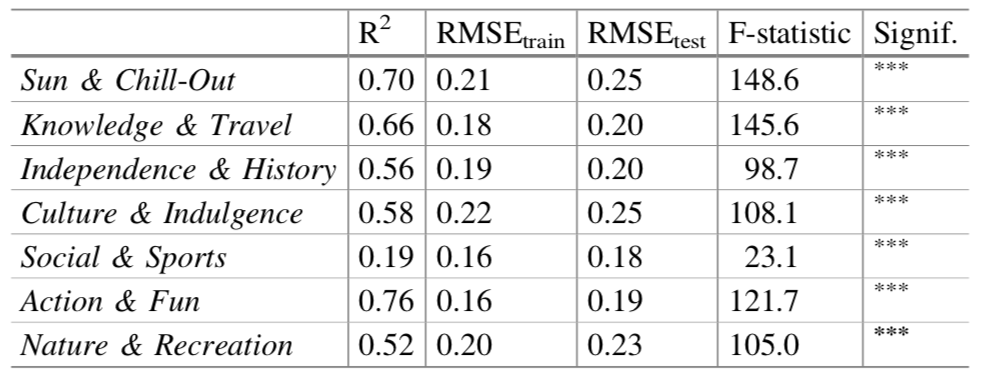
\includegraphics[width=\linewidth]{latex_files/figures/table3.png}
  \caption{Performance of the resulting multiple linear regression models \cite{sertkan2018mapping}}
  \label{fig:table3}
\end{figure}

					
The resulting models provide strong evidence that there lies a statistically significant relationship between selected destination features and the seven factors,(used in the corresponding models), with p < 0.001. The values of  RMSE\textsubscript{train} and RMSE\textsubscript{test} are close, indicating that the performance of the resulting models will be similar out of sample.  
					
Overall, all travel behavioural patterns are well described by the resulting models(52–76\% of the variance), except Social \& Sports, where only 19\% of the variance is explained. This can be accorded to the uneven distribution of the expert mapping of Social \& Sports, where 53.83\% of the destination scored with 0.5 and only 1.78\% scored with 0 and 4.10\% with 1 respectively.

However, there is significant evidence of a relationship between the destination features and the factor Social \& Sports. 70 and 76\% of the variance can be explained respectively for Sun \& Chill-Out and Action-Fun, making them the best fitted models
				
				




  
\section{Conclusion}

% \appendix
% %Appendix A
% \section{The Author}
% Ashmi Banerjee, currently a masters student in the department of Informatics at Technical University of Munich, received her Bachelor\textquotesingle s degree in Computer Science and Engineering from Heritage Institute of Technology, Kolkata, India.

% This paper was written as a part of an assignment during the Master-Seminar course 'Current Topics in Recommender Systems', organized by the Chair of
% Connected Mobility,during the winter semester 2018-19, at the Technical University of Munich.

% \section{Acknowledgement}